\documentclass[10pt]{article}
\usepackage{tikz}
\usepackage[margin=0cm]{geometry}
\pagestyle{empty}

\begin{document}

\vspace*{\fill}
\begin{center}
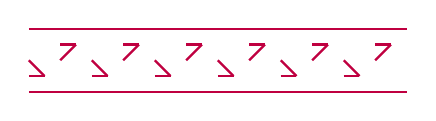
\begin{tikzpicture}[x=0.2cm, y=-0.2cm, thick, purple]
% North to South lines
% North-West to South-East lines
    \draw (0,2) -- (1,3);
    \draw (4,2) -- (5,3);
    \draw (8,2) -- (9,3);
    \draw (12,2) -- (13,3);
    \draw (16,2) -- (17,3);
    \draw (20,2) -- (21,3);
% West to East lines
    \draw (0,0) -- (24,0);
    \draw (2,1) -- (3,1);
    \draw (6,1) -- (7,1);
    \draw (10,1) -- (11,1);
    \draw (14,1) -- (15,1);
    \draw (18,1) -- (19,1);
    \draw (22,1) -- (23,1);
    \draw (0,3) -- (1,3);
    \draw (4,3) -- (5,3);
    \draw (8,3) -- (9,3);
    \draw (12,3) -- (13,3);
    \draw (16,3) -- (17,3);
    \draw (20,3) -- (21,3);
    \draw (0,4) -- (24,4);
% South-West to North-East lines
    \draw (2,2) -- (3,1);
    \draw (6,2) -- (7,1);
    \draw (10,2) -- (11,1);
    \draw (14,2) -- (15,1);
    \draw (18,2) -- (19,1);
    \draw (22,2) -- (23,1);
\end{tikzpicture}
\end{center}
\vspace*{\fill}

\end{document}
